% =============================================================================
% Chest Xpert AI - Serving a Multi-Label Chest Pathology Classifier
% Models in Production - UNI 2026
% =============================================================================
\documentclass[11pt, a4paper]{article}

% --- Core Packages ---
\usepackage[utf8]{inputenc}
\usepackage[T1]{fontenc}

% Use spanish for captions and content
\usepackage[spanish]{babel}

% Layout and margins
\usepackage[top=2.5cm, bottom=2.5cm, left=2.5cm, right=2.5cm]{geometry}

% Reduce whitespace around sections and floats
\usepackage{titlesec}
\titlespacing*{\section}{0pt}{12pt plus 4pt minus 2pt}{6pt plus 2pt}
\titlespacing*{\subsection}{0pt}{8pt plus 3pt minus 2pt}{4pt plus 2pt}

% Graphics and figures
\usepackage{graphicx}
\usepackage{float}
\usepackage[font=small, labelfont=bf, skip=6pt]{caption}

% Tables
\usepackage{booktabs}
\usepackage{tabularx}
\usepackage{array}

% Lists (compact)
\usepackage{enumitem}
\setlist{nosep, leftmargin=*, topsep=4pt, parsep=2pt, itemsep=2pt}

% Mathematics and symbols
\usepackage{amsmath}
\usepackage{amssymb}

% Code listings
\usepackage{listings}
\usepackage{xcolor}

\definecolor{codebg}{RGB}{245, 245, 245}
\definecolor{codegreen}{RGB}{40, 167, 69}
\definecolor{codegray}{RGB}{128, 128, 128}
\definecolor{codeblue}{RGB}{0, 123, 255}

\lstset{
    backgroundcolor=\color{codebg},
    basicstyle=\ttfamily\small,
    breaklines=true,
    frame=single,
    rulecolor=\color{codegray},
    numbers=left,
    numberstyle=\tiny\color{codegray},
    keywordstyle=\color{codeblue}\bfseries,
    commentstyle=\color{codegreen}\itshape,
    stringstyle=\color{red!70!black},
    showstringspaces=false,
    tabsize=2,
    captionpos=b
}

% Colors and links
\usepackage[hidelinks]{hyperref}
\usepackage{url}

% Bibliography
\usepackage[numbers, sort&compress]{natbib}
\setlength{\bibsep}{4pt}

% Headers and footers
\usepackage{fancyhdr}
\pagestyle{fancy}
\fancyhf{}
\fancyhead[L]{\footnotesize Chest Xpert AI -- Modelos en Producci\'on}
\fancyhead[R]{\footnotesize \thepage}
\renewcommand{\headrulewidth}{0.4pt}

% Prevent vertical stretching
\raggedbottom

% Abstract formatting
\usepackage{abstract}
\setlength{\absleftindent}{0pt}
\setlength{\absrightindent}{0pt}
\renewcommand{\abstractnamefont}{\normalfont\bfseries}
\renewcommand{\abstracttextfont}{\normalfont\small}

% =============================================================================
% DOCUMENT METADATA
% =============================================================================
\title{
    \vspace{-1.5cm}
    \Large\textbf{Chest Xpert AI: Despliegue de un Clasificador Multi-Etiqueta de Patolog\'ias Tor\'acicas como Servicio Containerizado} \\[0.3cm]
    \normalsize\normalfont Modelos en Producci\'on --- Programa de Especializaci\'on en IA Generativa y MLOps --- UNI 2026
}

\author{
    \textbf{Angel Eduardo Hincho Jove} \\[0.1cm]
    \small Universidad Nacional de Ingenier\'ia \\
    \small\texttt{ahincho@unsa.edu.pe}
}

\date{\small\today}

% =============================================================================
% DOCUMENT START
% =============================================================================
\begin{document}

\maketitle
\vspace{-0.5cm}

% =============================================================================
% RESUMEN
% =============================================================================
\begin{abstract}
\noindent
\textbf{Resumen.}
El presente trabajo documenta el proceso de despliegue en producci\'on de un modelo de clasificaci\'on multi-etiqueta de patolog\'ias tor\'acicas. El modelo, basado en DenseNet121 con transfer learning especializado mediante TorchXRayVision, detecta simult\'aneamente cinco patolog\'ias urgentes (Cardiomegaly, Edema, Consolidation, Atelectasis, Pleural Effusion) a partir de radiograf\'ias de t\'orax, alcanzando un AUC de 0.869. Se implement\'o una API REST con FastAPI y ONNX Runtime para inferencia eficiente ($\sim$20ms por predicci\'on), empaquetada en una imagen Docker multi-stage optimizada con usuario no-root y modelo embebido. Se configur\'o un pipeline completo de CI/CD con GitHub Actions que incluye linting (Ruff), testing (pytest), versionado sem\'antico autom\'atico y publicaci\'on de la imagen en GitHub Container Registry. El servicio se levanta con un solo comando \texttt{docker run} sin dependencias externas.

\vspace{0.3cm}
\noindent
\textbf{Palabras clave:} Docker, FastAPI, ONNX Runtime, CI/CD, GitHub Actions, GHCR, Deep Learning, clasificaci\'on multi-etiqueta, MLOps, versionado sem\'antico.
\end{abstract}


% --- Sections ---
% =============================================================================
% 1. INTRODUCCION
% =============================================================================
\section{Introducci\'on}
\label{sec:introduction}

\subsection{Contexto del modelo original}

En un trabajo previo se desarroll\'o \textbf{Chest Xpert AI}, un sistema de clasificaci\'on autom\'atica multi-etiqueta de cinco patolog\'ias tor\'acicas urgentes---Cardiomegaly, Edema, Consolidation, Atelectasis y Pleural Effusion---a partir de radiograf\'ias frontales de t\'orax \cite{irvin2019chexpert}. El sistema utiliza una arquitectura DenseNet121 \cite{huang2017densenet} con transfer learning especializado mediante TorchXRayVision \cite{cohen2022torchxrayvision}, un backbone preentrenado en m\'as de 500,000 radiograf\'ias reales, alcanzando un AUC macro de 0.869 [IC 95\%: 0.844--0.893].

El modelo fue exportado a formato ONNX con normalizaci\'on embebida, eliminando el training-serving skew y permitiendo inferencia en aproximadamente 20ms sin dependencia de PyTorch en producci\'on.

\begin{figure}[H]
    \centering
    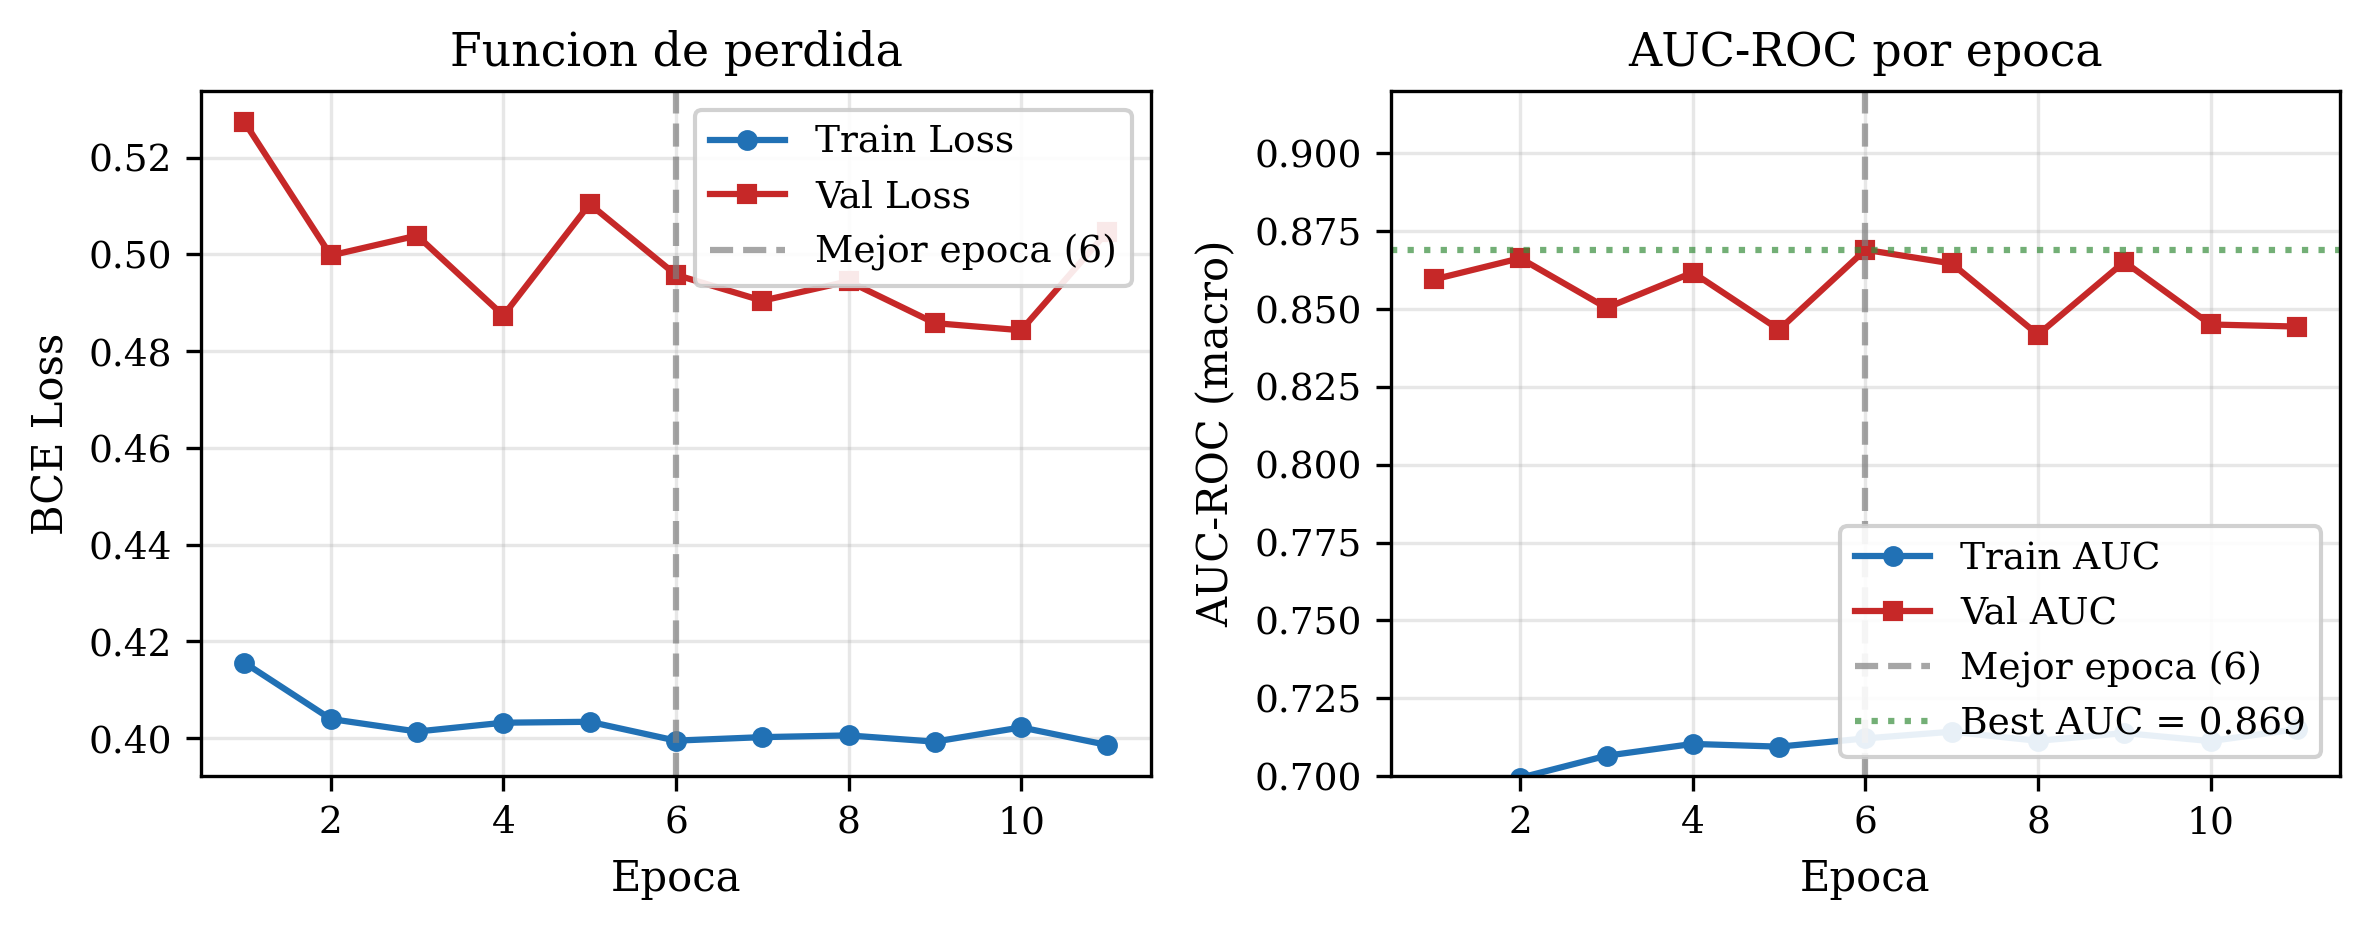
\includegraphics[width=0.85\textwidth]{figures/training-curves.png}
    \caption{Curvas de entrenamiento del modelo original: loss y AUC por \'epoca. Early Stopping activado en \'epoca 11; mejor modelo restaurado de \'epoca 6.}
    \label{fig:training}
\end{figure}

\subsection{Motivaci\'on: del notebook a producci\'on}

Existe una brecha significativa entre desarrollar un modelo de Machine Learning en un notebook y desplegarlo como servicio confiable \cite{sculley2015technical}. Los principales desaf\'ios incluyen:

\begin{itemize}
    \item \textbf{Reproducibilidad}: el modelo debe comportarse id\'enticamente en cualquier m\'aquina.
    \item \textbf{Aislamiento}: las dependencias del modelo no deben interferir con el sistema host.
    \item \textbf{Escalabilidad}: el servicio debe poder desplegarse en cualquier infraestructura cloud.
    \item \textbf{Confiabilidad}: cada cambio debe pasar por validaciones autom\'aticas antes de producción.
\end{itemize}

La containerizaci\'on con Docker y los pipelines de CI/CD resuelven estos desaf\'ios de forma est\'andar en la industria \cite{gift2021mlops}.

\subsection{Objetivo}

Empaquetar el modelo Chest Xpert AI como un servicio HTTP containerizado que:
\begin{enumerate}
    \item Arranque con un solo comando (\texttt{docker run}).
    \item Reciba una radiograf\'ia de t\'orax y devuelva predicciones de cinco patolog\'ias.
    \item Aplique las mejores pr\'acticas de Docker, CI/CD y MLOps vigentes en 2026.
    \item Se publique autom\'aticamente en un registry p\'ublico (GHCR).
\end{enumerate}

\begin{figure}[H]
    \centering
    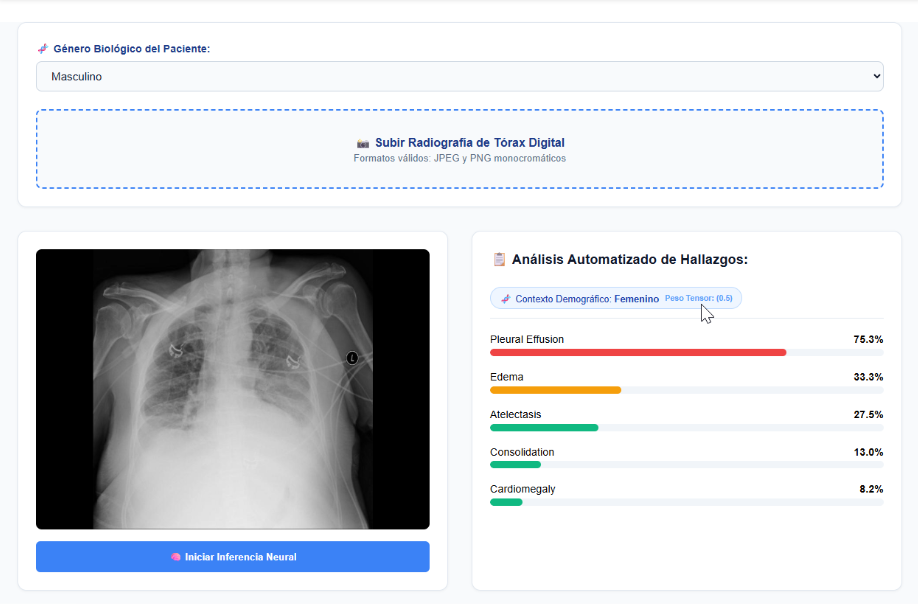
\includegraphics[width=0.85\textwidth]{figures/fullstack-plus-model-application.png}
    \caption{Arquitectura general del ecosistema Chest Xpert AI: modelo de entrenamiento, backend (FastAPI + ONNX), y frontend (Angular).}
    \label{fig:fullstack}
\end{figure}

% =============================================================================
% 2. ARQUITECTURA DE LA SOLUCION
% =============================================================================
\section{Arquitectura de la soluci\'on}
\label{sec:architecture}

\subsection{Visi\'on general}

El sistema sigue una arquitectura de microservicio stateless donde el cliente env\'ia una imagen y recibe predicciones en formato JSON. Los componentes principales son:

\begin{enumerate}
    \item \textbf{Cliente}: cualquier aplicaci\'on que realice requests HTTP (curl, frontend Angular, Postman).
    \item \textbf{API REST (FastAPI)}: recibe la imagen, la valida, la preprocesa y orquesta la inferencia.
    \item \textbf{Motor de inferencia (ONNX Runtime)}: ejecuta el modelo DenseNet121 exportado.
    \item \textbf{Contenedor Docker}: empaqueta todo en una unidad portable y reproducible.
\end{enumerate}

\subsection{Flujo de datos}

El procesamiento de una solicitud sigue estos pasos:

\begin{enumerate}
    \item El cliente env\'ia un \texttt{POST /predict} con la imagen en formato \texttt{multipart/form-data}.
    \item El \textbf{FilterService} valida que la imagen sea una radiograf\'ia (grayscale) mediante an\'alisis de varianza RGB. Im\'agenes a color son rechazadas.
    \item El \textbf{PreprocessingService} convierte la imagen a escala de grises, la redimensiona a $224 \times 224$ p\'ixeles y la transforma en un tensor float32 de forma $(1, 1, 224, 224)$.
    \item El \textbf{InferenceService} ejecuta el modelo ONNX y obtiene 5 probabilidades independientes.
    \item La API devuelve un JSON con las predicciones por patolog\'ia.
\end{enumerate}

\subsection{Decisiones de dise\~no}

La Tabla~\ref{tab:design-decisions} resume las decisiones t\'ecnicas clave:

\begin{table}[H]
\centering
\caption{Decisiones de dise\~no del servicio.}
\label{tab:design-decisions}
\small
\begin{tabularx}{\textwidth}{lX}
\toprule
\textbf{Decisi\'on} & \textbf{Justificaci\'on} \\
\midrule
FastAPI & Framework async, documentaci\'on autom\'atica (OpenAPI), validaci\'on con Pydantic \\
ONNX Runtime & Reemplaza PyTorch ($\sim$2GB) por un runtime liviano ($\sim$50MB), inferencia en $\sim$20ms \\
uv (gestor de deps) & Resoluci\'on 10--100x m\'as r\'apida que pip, lockfile determinista \\
Multi-stage Docker & Separa build de runtime, reduce tama\~no de imagen \\
Modelo embebido & Arranca con \texttt{docker run} sin vol\'umenes ni configuraci\'on \\
Usuario no-root & Principio de m\'inimo privilegio, requerido en entornos productivos \\
\bottomrule
\end{tabularx}
\end{table}

\subsection{Estructura del proyecto}

\begin{lstlisting}[language={}, caption={Estructura del repositorio chest-xpert-backend.}]
chest-xpert-backend/
+-- .github/workflows/
|   +-- ci.yml              # Lint + Test + Build + Release
|   +-- cd.yml              # Build + Push a GHCR
+-- app/
|   +-- main.py             # App factory + lifespan
|   +-- config.py           # Settings (pydantic-settings)
|   +-- routers/
|   |   +-- health.py       # GET /health
|   |   +-- predict.py      # POST /predict
|   +-- schemas/
|   |   +-- prediction.py   # Request/Response models
|   +-- services/
|       +-- inference.py    # ONNX Runtime session
|       +-- preprocessing.py # Imagen -> tensor
|       +-- filter.py       # Filtro RGB-Diff
+-- models/                  # Modelo ONNX (embebido en imagen)
+-- tests/                   # pytest + Hypothesis
+-- Dockerfile               # Multi-stage production build
+-- pyproject.toml           # Deps + Ruff + Semantic Release
+-- uv.lock                  # Lockfile determinista
\end{lstlisting}

% =============================================================================
% 3. IMPLEMENTACION
% =============================================================================
\section{Implementaci\'on}
\label{sec:implementation}

\subsection{API REST con FastAPI}

La API expone dos endpoints principales:

\begin{itemize}
    \item \texttt{GET /health}: verificaci\'on de estado del servicio.
    \item \texttt{POST /predict}: clasificaci\'on de radiograf\'ia de t\'orax (acepta JPEG/PNG, m\'aximo 10MB).
\end{itemize}

El ciclo de vida de la aplicaci\'on gestiona la carga del modelo ONNX al iniciar y su liberaci\'on al apagar:

\begin{lstlisting}[language=Python, caption={Lifespan del modelo ONNX en FastAPI.}]
@asynccontextmanager
async def lifespan(app: FastAPI):
    settings: Settings = app.state.settings
    try:
        app.state.inference_service = InferenceService(
            settings.model_path
        )
    except FileNotFoundError as exc:
        raise SystemExit(1) from exc
    yield
    app.state.inference_service.close()
\end{lstlisting}

\subsection{Servicio de inferencia}

El modelo se carga una sola vez al arrancar y se reutiliza para todas las solicitudes:

\begin{lstlisting}[language=Python, caption={InferenceService con ONNX Runtime.}]
class InferenceService:
    def __init__(self, model_path: str) -> None:
        path = Path(model_path)
        if not path.is_file():
            raise FileNotFoundError(f"Model not found: {model_path}")
        self.session = ort.InferenceSession(model_path)

    def predict(self, tensor: NDArray[np.float32]):
        results = self.session.run(
            ["predictions"], {"image": tensor}
        )
        return results[0][0]  # 5 probabilidades
\end{lstlisting}

La entrada es un tensor float32 de forma $(1, 1, 224, 224)$ con valores de p\'ixel en $[0, 255]$. El modelo maneja la normalizaci\'on internamente (normalizaci\'on embebida en ONNX), eliminando el riesgo de training-serving skew.

\begin{figure}[H]
    \centering
    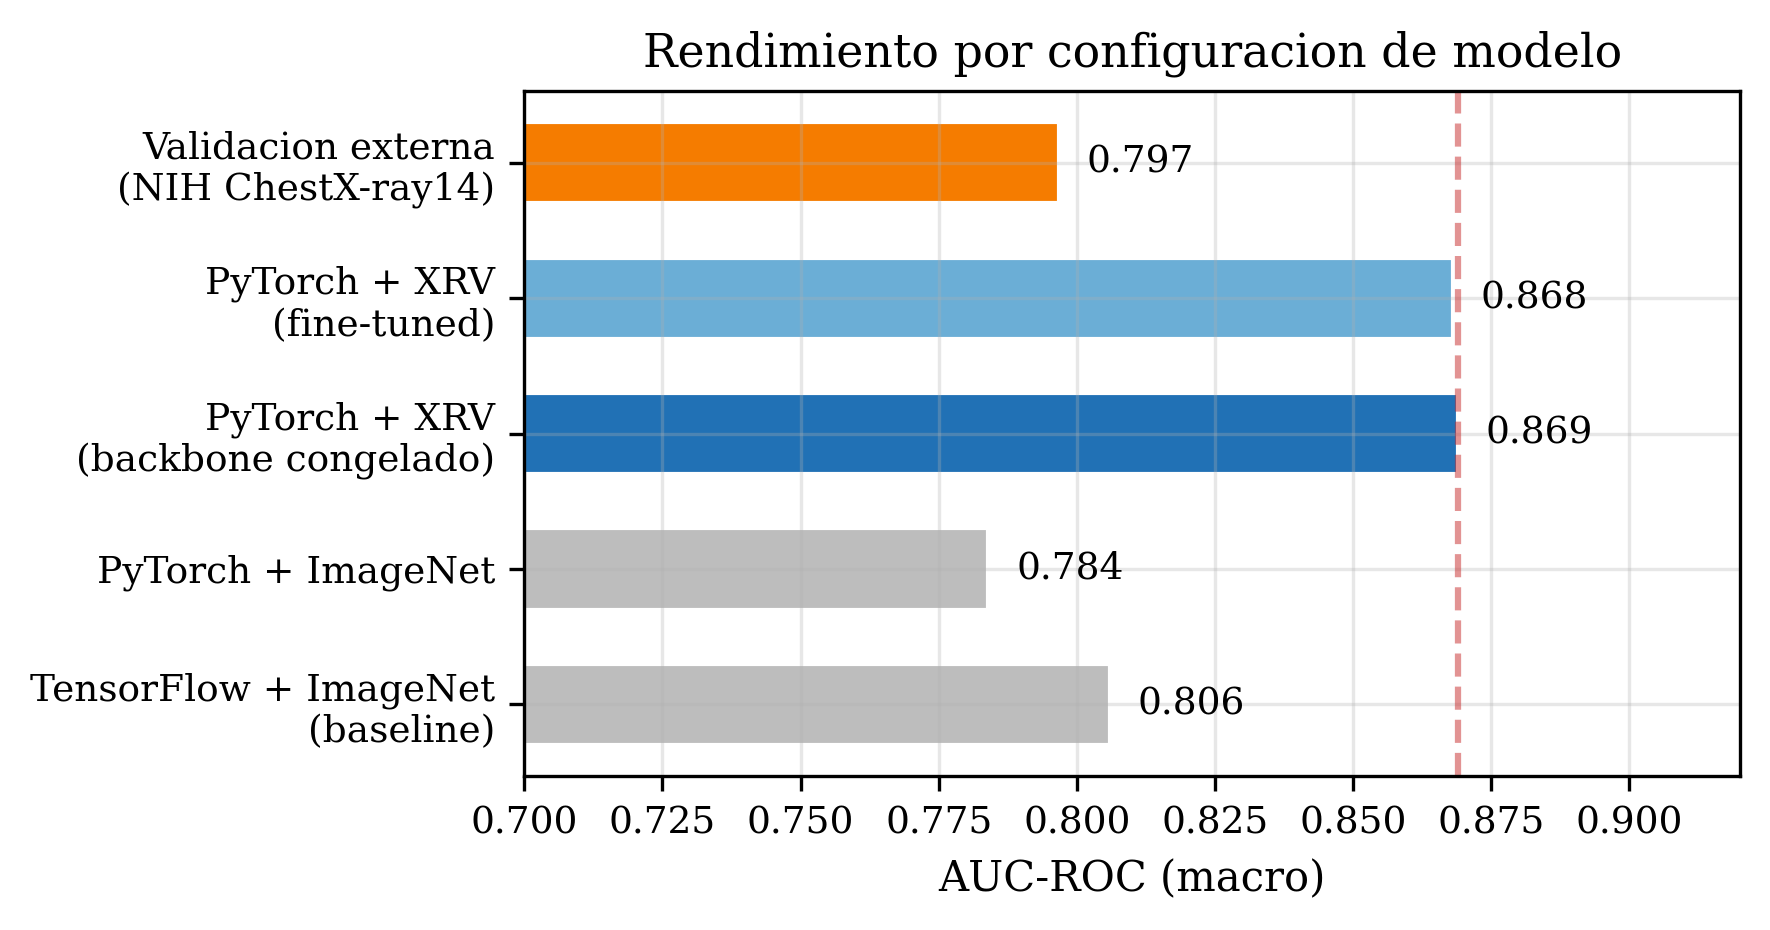
\includegraphics[width=0.85\textwidth]{figures/auc-roc-model-configs.png}
    \caption{Curvas AUC-ROC por patolog\'ia del modelo DenseNet121 + TorchXRayVision. AUC macro = 0.869.}
    \label{fig:auc-roc}
\end{figure}

\subsection{Dockerfile multi-stage}

El Dockerfile aplica las mejores pr\'acticas de producci\'on vigentes en 2026:

\begin{lstlisting}[language={}, caption={Dockerfile multi-stage (simplificado).}]
# Stage 1: Build
FROM python:3.14-slim-bookworm AS builder
COPY --from=ghcr.io/astral-sh/uv:0.11.21 /uv /bin/
ENV UV_COMPILE_BYTECODE=1
ENV UV_LINK_MODE=copy
WORKDIR /build
COPY pyproject.toml uv.lock ./
RUN uv sync --frozen --no-dev --no-install-project
COPY app/ ./app/
RUN uv sync --frozen --no-dev --no-editable

# Stage 2: Runtime
FROM python:3.14-slim-bookworm AS runtime
RUN groupadd -r chest-xpert && useradd -r -g chest-xpert ...
COPY --from=builder --chown=chest-xpert:chest-xpert \
    /build/.venv /app/.venv
COPY --chown=chest-xpert:chest-xpert models/ ./models/
USER chest-xpert
HEALTHCHECK CMD ["python", "-c", "...urlopen(health)..."]
CMD ["python", "-m", "uvicorn", "app.main:app", ...]
\end{lstlisting}

\noindent
Pr\'acticas aplicadas en el Dockerfile:

\begin{itemize}
    \item \textbf{Multi-stage build}: separa dependencias de compilaci\'on del runtime final.
    \item \textbf{UV pinned} (v0.11.21): resoluci\'on r\'apida y determinista de dependencias.
    \item \textbf{Bytecode precompilado} (\texttt{UV\_COMPILE\_BYTECODE=1}): startup m\'as r\'apido.
    \item \textbf{Cache mounts}: builds incrementales eficientes en CI.
    \item \textbf{Intermediate layers}: dependencias y c\'odigo en capas separadas para cache \'optima.
    \item \textbf{Non-root user}: principio de m\'inimo privilegio.
    \item \textbf{Modelo embebido}: no requiere vol\'umenes para arrancar.
    \item \textbf{OCI Labels}: metadata para trazabilidad con \texttt{docker inspect}.
    \item \textbf{HEALTHCHECK}: integraci\'on con orquestadores (Docker, ECS, Kubernetes).
\end{itemize}

\subsection{Gesti\'on de configuraci\'on}

La configuraci\'on se maneja con \texttt{pydantic-settings}, cargando valores desde variables de entorno con prefijo \texttt{CHEST\_XPERT\_}:

\begin{table}[H]
\centering
\caption{Variables de configuraci\'on del servicio.}
\small
\begin{tabular}{llp{5cm}}
\toprule
\textbf{Variable} & \textbf{Default} & \textbf{Descripci\'on} \\
\midrule
\texttt{MODEL\_PATH} & \texttt{models/...onnx} & Ruta al modelo ONNX \\
\texttt{SERVER\_PORT} & 8000 & Puerto del servidor \\
\texttt{RGB\_DIFF\_THRESHOLD} & 5.0 & Umbral del filtro de seguridad \\
\texttt{CORS\_ORIGINS} & localhost:4200 & Or\'igenes CORS permitidos \\
\bottomrule
\end{tabular}
\end{table}

Nunca se incluyen secretos dentro de la imagen. Las API keys se inyectan en runtime mediante \texttt{-e} o archivos \texttt{.env} montados.

% =============================================================================
% 4. DESPLIEGUE Y ENTREGA CONTINUA
% =============================================================================
\section{Despliegue y entrega continua}
\label{sec:deployment}

\subsection{Pipeline de CI (Integraci\'on Continua)}

El pipeline de CI se ejecuta en cada push a \texttt{main} y en cada Pull Request. Consta de cuatro jobs secuenciales:

\begin{enumerate}
    \item \textbf{Lint (Ruff)}: verifica estilo de c\'odigo y detecta errores com\'unes (15 conjuntos de reglas activos).
    \item \textbf{Test (pytest)}: ejecuta la suite de tests unitarios con cobertura.
    \item \textbf{Build (Docker)}: verifica que el Dockerfile compila correctamente sin hacer push.
    \item \textbf{Semantic Release}: analiza los commits convencionales, bumps la versi\'on y crea un tag Git autom\'aticamente.
\end{enumerate}

\begin{lstlisting}[language={}, caption={Fragmento de ci.yml --- Job de lint.}]
lint:
  name: Lint (ruff)
  runs-on: ubuntu-latest
  steps:
    - uses: actions/checkout@v6
    - uses: astral-sh/setup-uv@v8.2.0
    - run: uv python install 3.14
    - run: uv sync --frozen --extra dev
    - run: uv run ruff check .
    - run: uv run ruff format --check .
\end{lstlisting}

\subsection{Pipeline de CD (Entrega Continua)}

El pipeline de CD se dispara cuando se crea un tag sem\'antico (\texttt{v*.*.*}). Construye la imagen Docker y la publica en GitHub Container Registry:

\begin{lstlisting}[language={}, caption={Fragmento de cd.yml --- Build y push a GHCR.}]
on:
  push:
    tags: ["v*.*.*"]

jobs:
  build-and-push:
    steps:
      - uses: docker/login-action@v4
        with:
          registry: ghcr.io
          username: ${{ github.actor }}
          password: ${{ secrets.GITHUB_TOKEN }}
      - uses: docker/metadata-action@v6
        with:
          tags: |
            type=semver,pattern={{version}}
            type=semver,pattern={{major}}.{{minor}}
            type=raw,value=latest
            type=sha,prefix=sha-,format=short
      - uses: docker/build-push-action@v7
        with:
          push: true
          tags: ${{ steps.meta.outputs.tags }}
\end{lstlisting}

\noindent
Los tags generados para una release \texttt{v1.0.2} son:

\begin{itemize}
    \item \texttt{ghcr.io/ahincho/chest-xpert-backend:1.0.2}
    \item \texttt{ghcr.io/ahincho/chest-xpert-backend:1.0}
    \item \texttt{ghcr.io/ahincho/chest-xpert-backend:1}
    \item \texttt{ghcr.io/ahincho/chest-xpert-backend:latest}
    \item \texttt{ghcr.io/ahincho/chest-xpert-backend:sha-a953d13}
\end{itemize}

\subsection{Versionado sem\'antico autom\'atico}

Se utiliza \texttt{python-semantic-release} \cite{gift2021mlops} configurado en \texttt{pyproject.toml} para automatizar el versionado basado en Conventional Commits:

\begin{table}[H]
\centering
\caption{Convenci\'on de commits y efecto en la versi\'on.}
\small
\begin{tabular}{llp{4.5cm}}
\toprule
\textbf{Prefijo} & \textbf{Bump} & \textbf{Ejemplo} \\
\midrule
\texttt{fix:}   & Patch (1.0.0 $\rightarrow$ 1.0.1) & \texttt{fix: handle empty image} \\
\texttt{feat:}  & Minor (1.0.0 $\rightarrow$ 1.1.0) & \texttt{feat: add /metrics endpoint} \\
\texttt{feat!:} & Major (1.0.0 $\rightarrow$ 2.0.0) & \texttt{feat!: change response schema} \\
\texttt{chore:} & Sin release & \texttt{chore: update README} \\
\bottomrule
\end{tabular}
\end{table}

\subsection{Seguridad y buenas pr\'acticas}

\begin{itemize}
    \item \textbf{Sin secretos en el repositorio}: \texttt{.gitignore} excluye \texttt{.env}, \texttt{.dockerignore} excluye datos sensibles del build context.
    \item \textbf{GITHUB\_TOKEN autom\'atico}: no se requieren tokens personales; GitHub Actions provee un token efímero por cada ejecuci\'on.
    \item \textbf{Build provenance attestation}: cada imagen publicada incluye un certificado de origen verificable (supply chain security).
    \item \textbf{Linting obligatorio}: el c\'odigo no llega a producci\'on sin pasar Ruff (15 reglas incluyendo seguridad con Bandit).
\end{itemize}

% =============================================================================
% 5. OBSERVABILIDAD
% =============================================================================
\section{Observabilidad}
\label{sec:observability}

\subsection{Stack LGTM con OpenTelemetry}

Para monitorear el servicio en producci\'on se implement\'o un stack de observabilidad completo basado en el proyecto open-source \textbf{Grafana LGTM} (Loki, Grafana, Tempo, Mimir) con OpenTelemetry como capa de instrumentaci\'on. La Tabla~\ref{tab:observability-stack} describe cada componente:

\begin{table}[H]
\centering
\caption{Componentes del stack de observabilidad.}
\label{tab:observability-stack}
\small
\begin{tabularx}{\textwidth}{llX}
\toprule
\textbf{Componente} & \textbf{Se\~nal} & \textbf{Prop\'osito} \\
\midrule
Tempo      & Traces   & Tracing distribuido: latencia por endpoint, spans por request \\
Loki       & Logs     & Agregaci\'on de logs estructurados del backend \\
Mimir      & Metrics  & M\'etricas de rendimiento (throughput, latencia p95, errores) \\
Pyroscope  & Profiles & Profiling continuo de CPU/memoria (flame graphs) \\
Grafana    & ---      & Visualizaci\'on unificada de todas las se\~nales \\
OTel Collector & --- & Recepci\'on y enrutamiento de telemetr\'ia via OTLP \\
\bottomrule
\end{tabularx}
\end{table}

\subsection{Instrumentaci\'on del backend}

La instrumentaci\'on se implementó con el SDK de OpenTelemetry para Python, configurable din\'amicamente mediante la variable de entorno \texttt{OTEL\_ENABLED}:

\begin{itemize}
    \item \textbf{Traces}: auto-instrumentaci\'on de FastAPI genera spans por cada request HTTP con m\'etodo, ruta, status code y duraci\'on.
    \item \textbf{Logs}: el handler de OTel se conecta al \texttt{logging} de Python, exportando todos los logs INFO/WARNING/ERROR a Loki via OTLP.
    \item \textbf{Metrics}: m\'etricas HTTP est\'andar (request count, latencia, tama\~no) m\'as m\'etricas custom de negocio.
\end{itemize}

\noindent
M\'etricas custom implementadas:

\begin{itemize}
    \item \texttt{chest\_xpert.predictions\_total}: contador de predicciones realizadas.
    \item \texttt{chest\_xpert.inference\_duration\_seconds}: histograma de duraci\'on de inferencia ONNX.
\end{itemize}

\subsection{Despliegue con Docker Compose}

El stack se levanta con un solo comando mediante \texttt{docker compose up}, desplegando dos contenedores:

\begin{lstlisting}[language=bash, caption={Levantar el stack completo.}]
docker compose up -d
# API:     http://localhost:8000
# Grafana: http://localhost:3000 (admin/admin)
\end{lstlisting}

\begin{figure}[H]
    \centering
    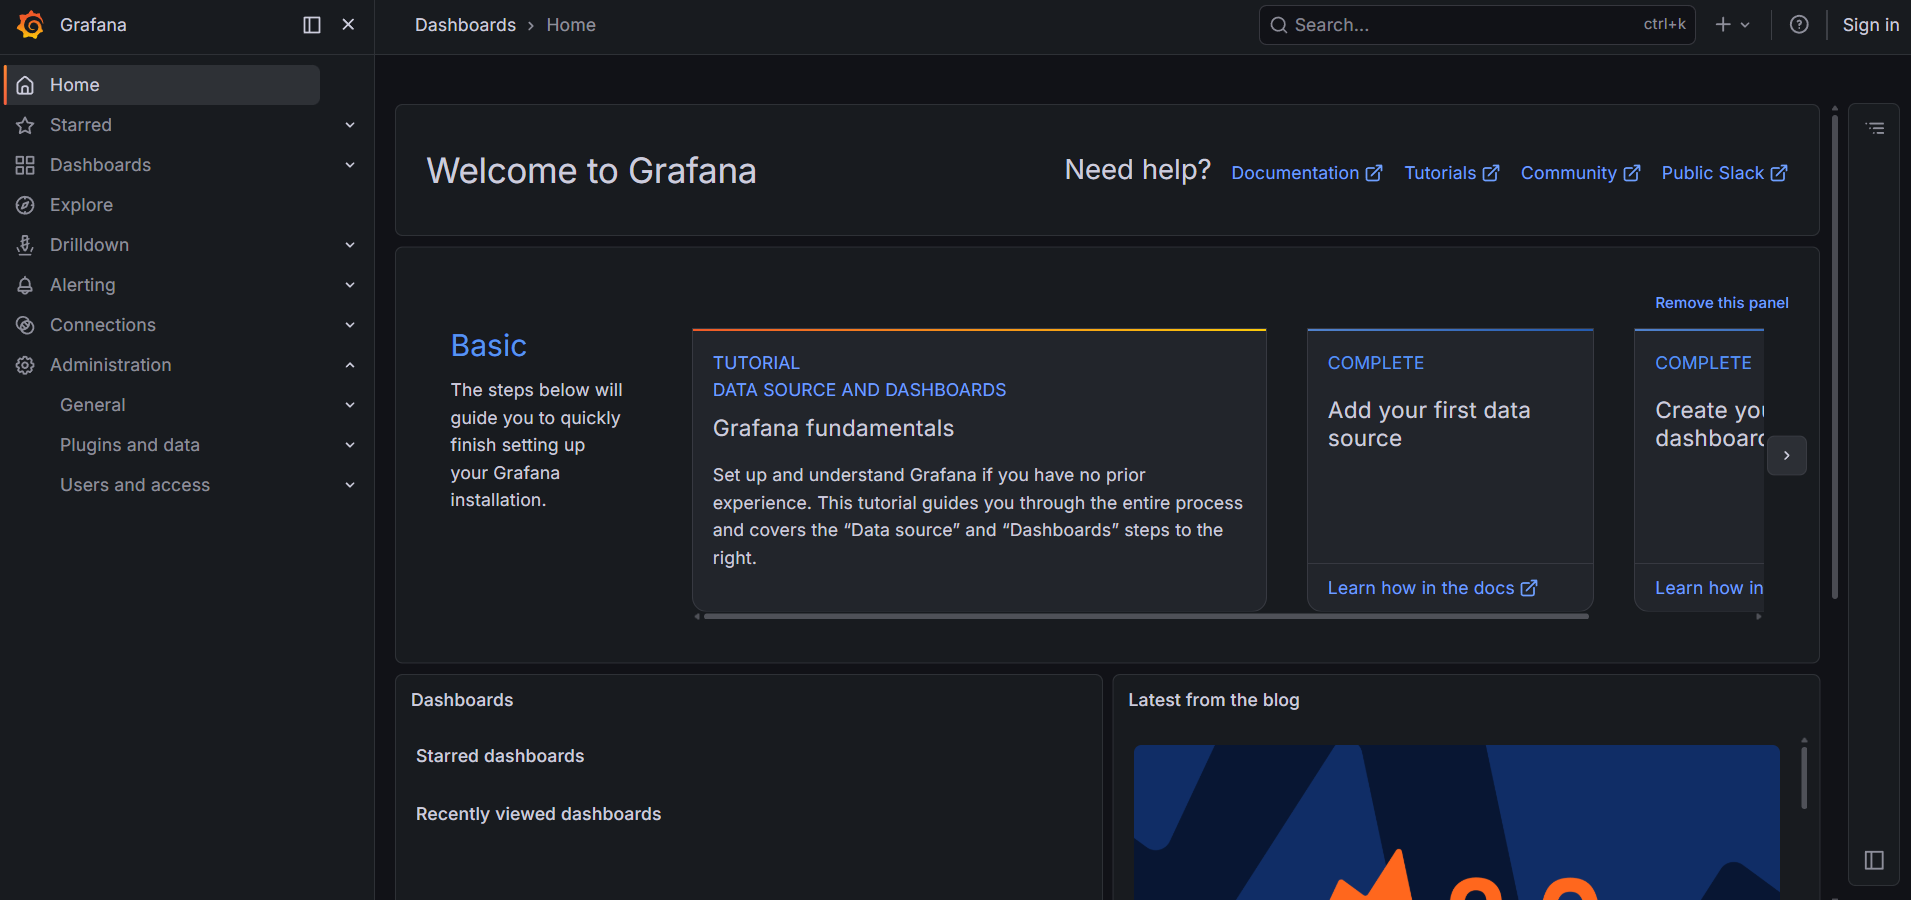
\includegraphics[width=0.9\textwidth]{figures/dashboard-grafana.png}
    \caption{Dashboard de Grafana con los datasources del stack LGTM configurados y recibiendo telemetr\'ia del backend.}
    \label{fig:dashboard-grafana}
\end{figure}

\subsection{Visualizaci\'on de se\~nales}

\begin{figure}[H]
    \centering
    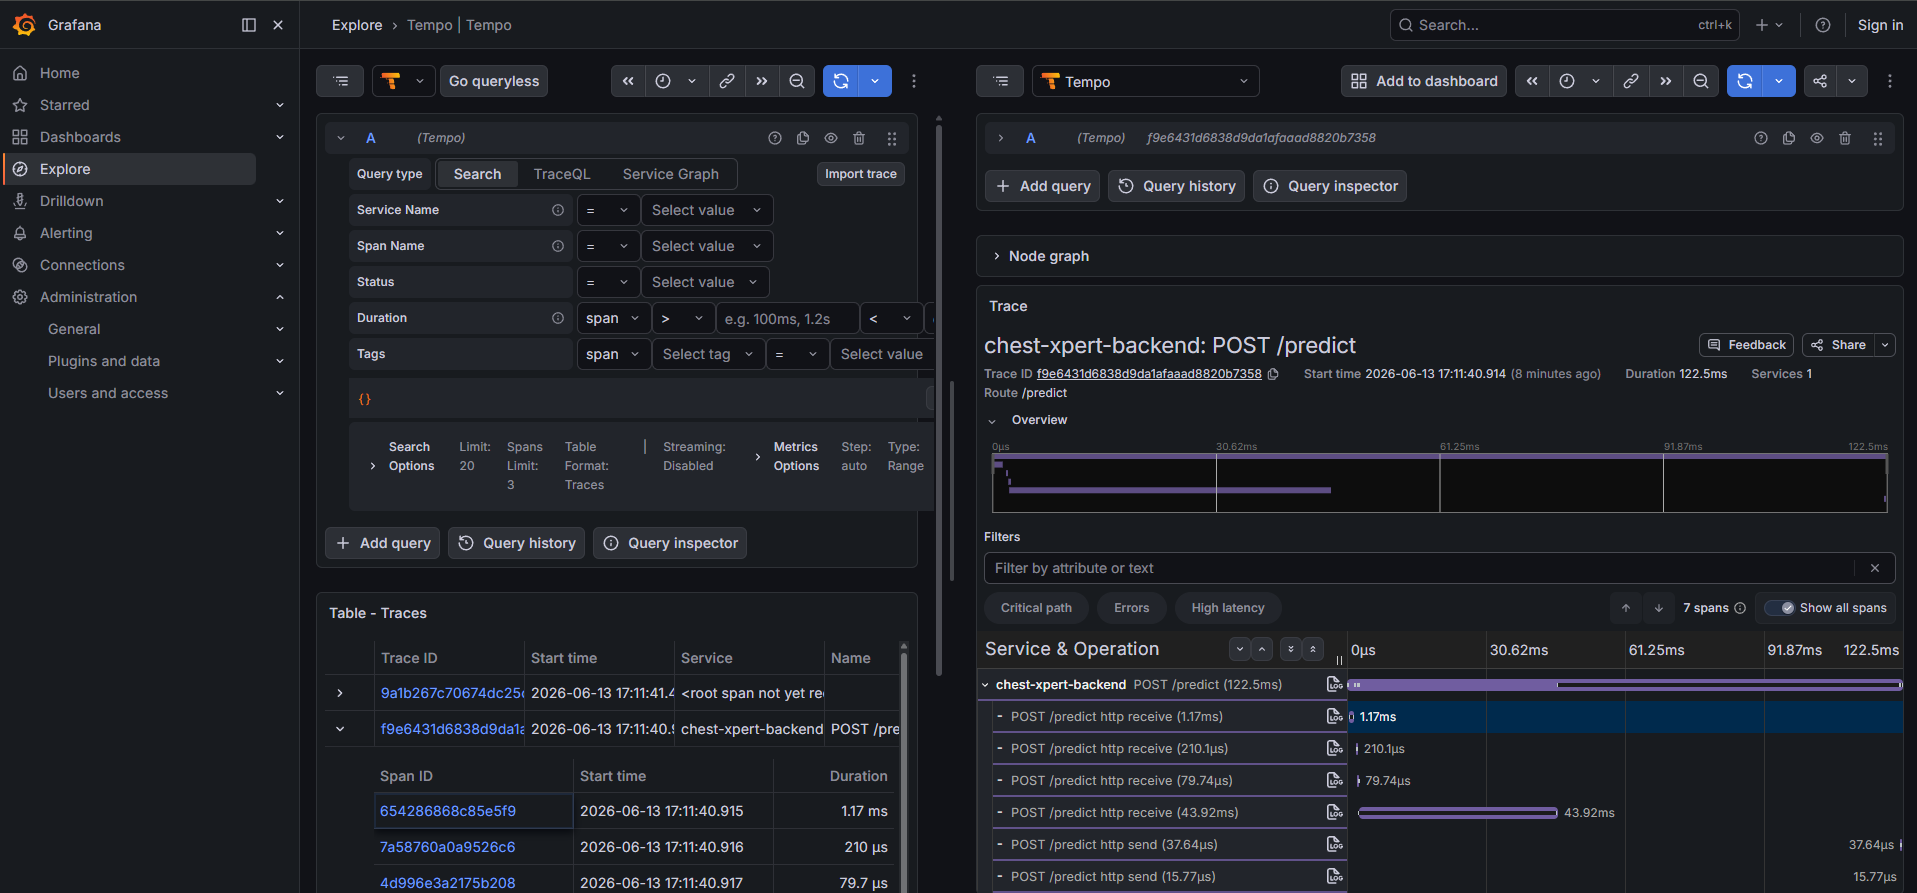
\includegraphics[width=0.9\textwidth]{figures/tempo.png}
    \caption{Tempo: traces distribuidos mostrando latencia por request al endpoint \texttt{/predict}. Cada trace incluye el span completo del ciclo request-response.}
    \label{fig:tempo}
\end{figure}

\begin{figure}[H]
    \centering
    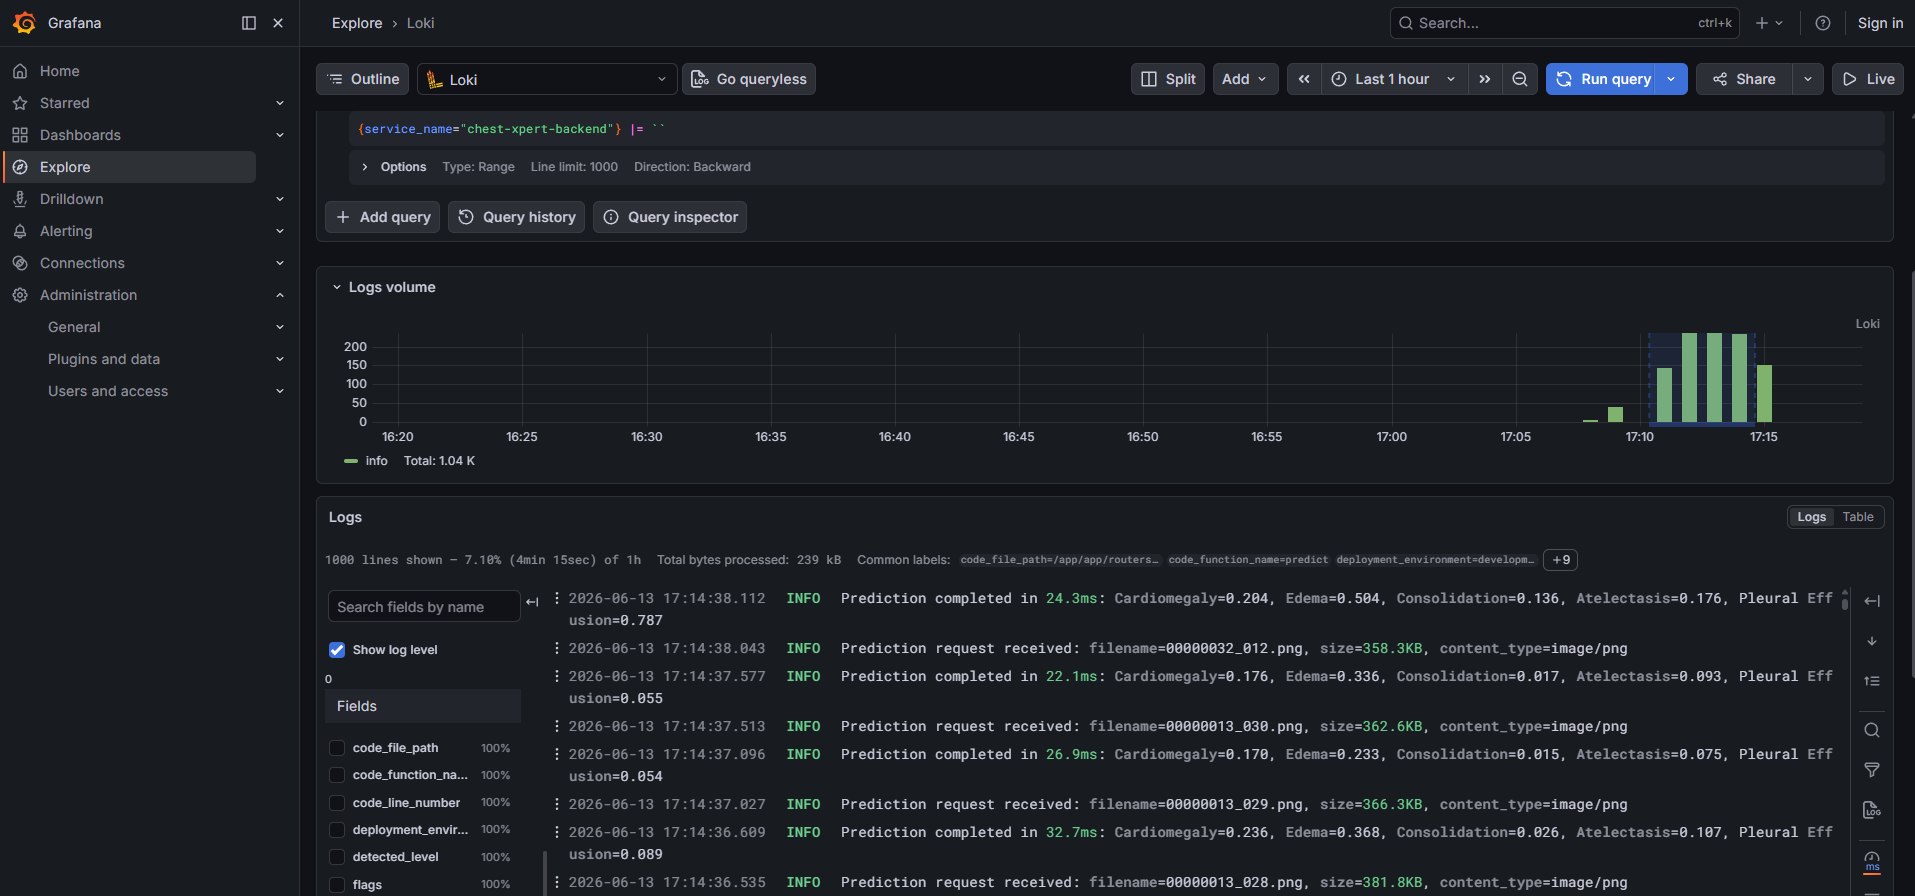
\includegraphics[width=0.9\textwidth]{figures/loki.png}
    \caption{Loki: logs estructurados del backend incluyendo filename, tama\~no, tiempo de inferencia y probabilidades por patolog\'ia.}
    \label{fig:loki}
\end{figure}

\begin{figure}[H]
    \centering
    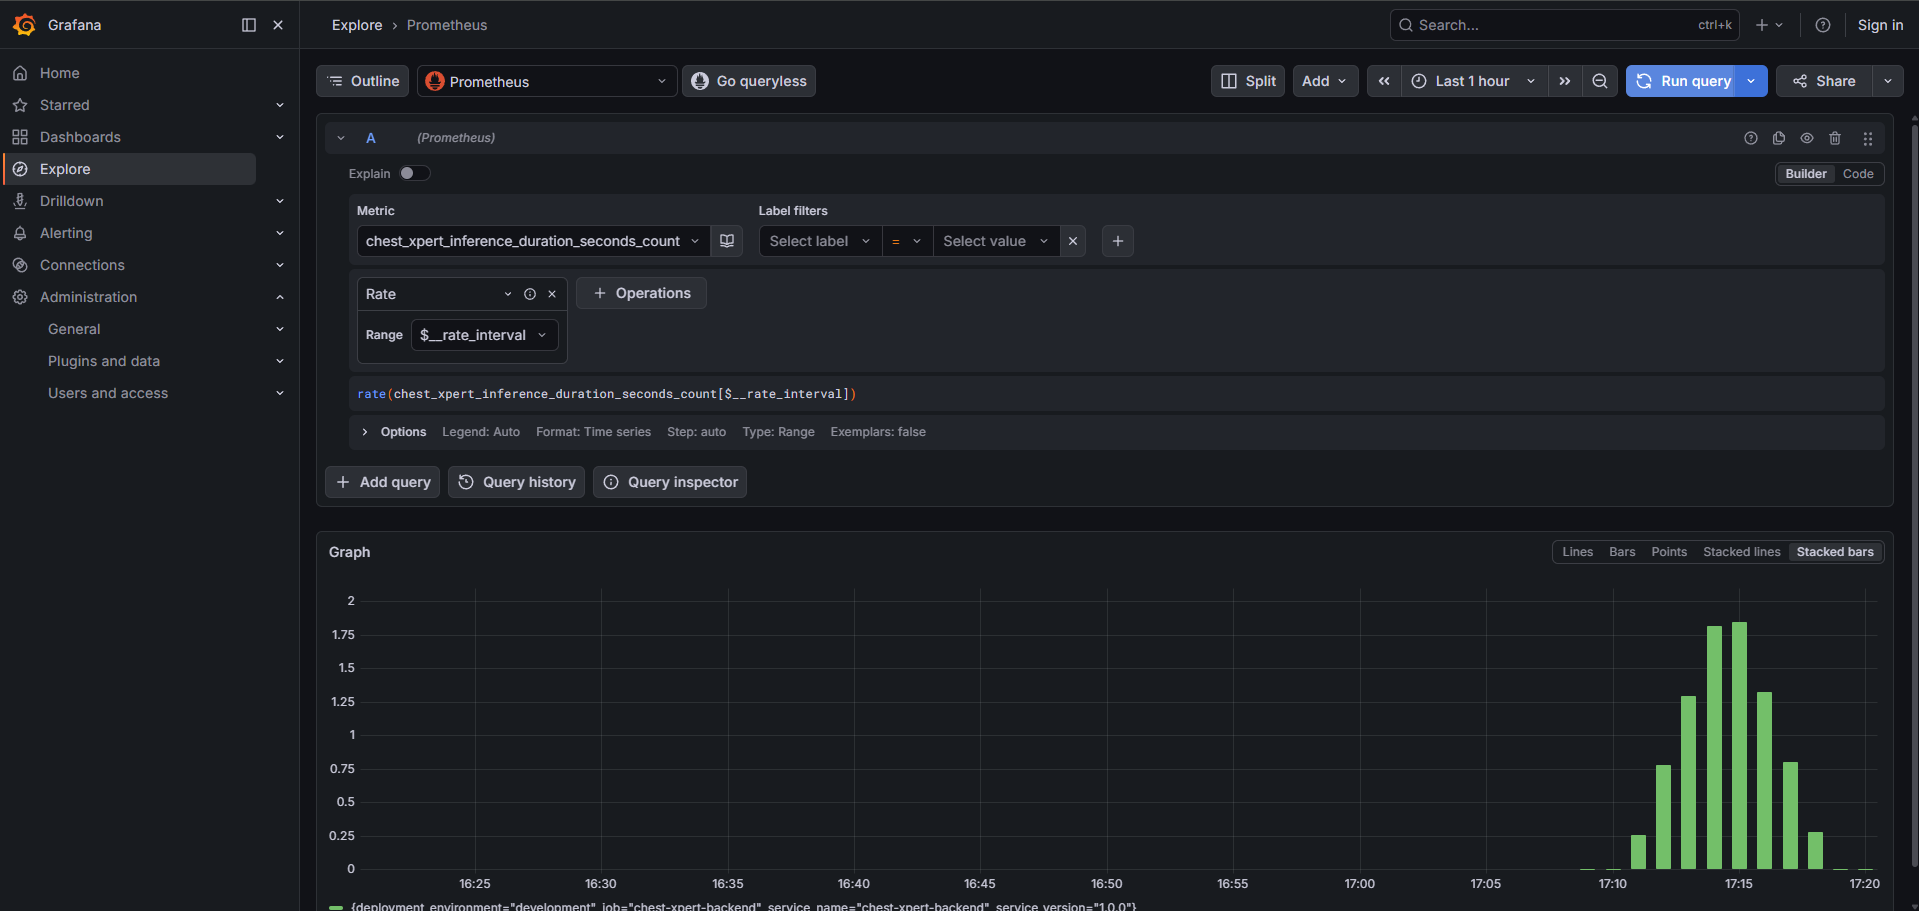
\includegraphics[width=0.9\textwidth]{figures/prometheus.png}
    \caption{Prometheus/Mimir: m\'etricas del servicio incluyendo \texttt{chest\_xpert.predictions\_total} y latencia de inferencia ONNX.}
    \label{fig:prometheus}
\end{figure}

\begin{figure}[H]
    \centering
    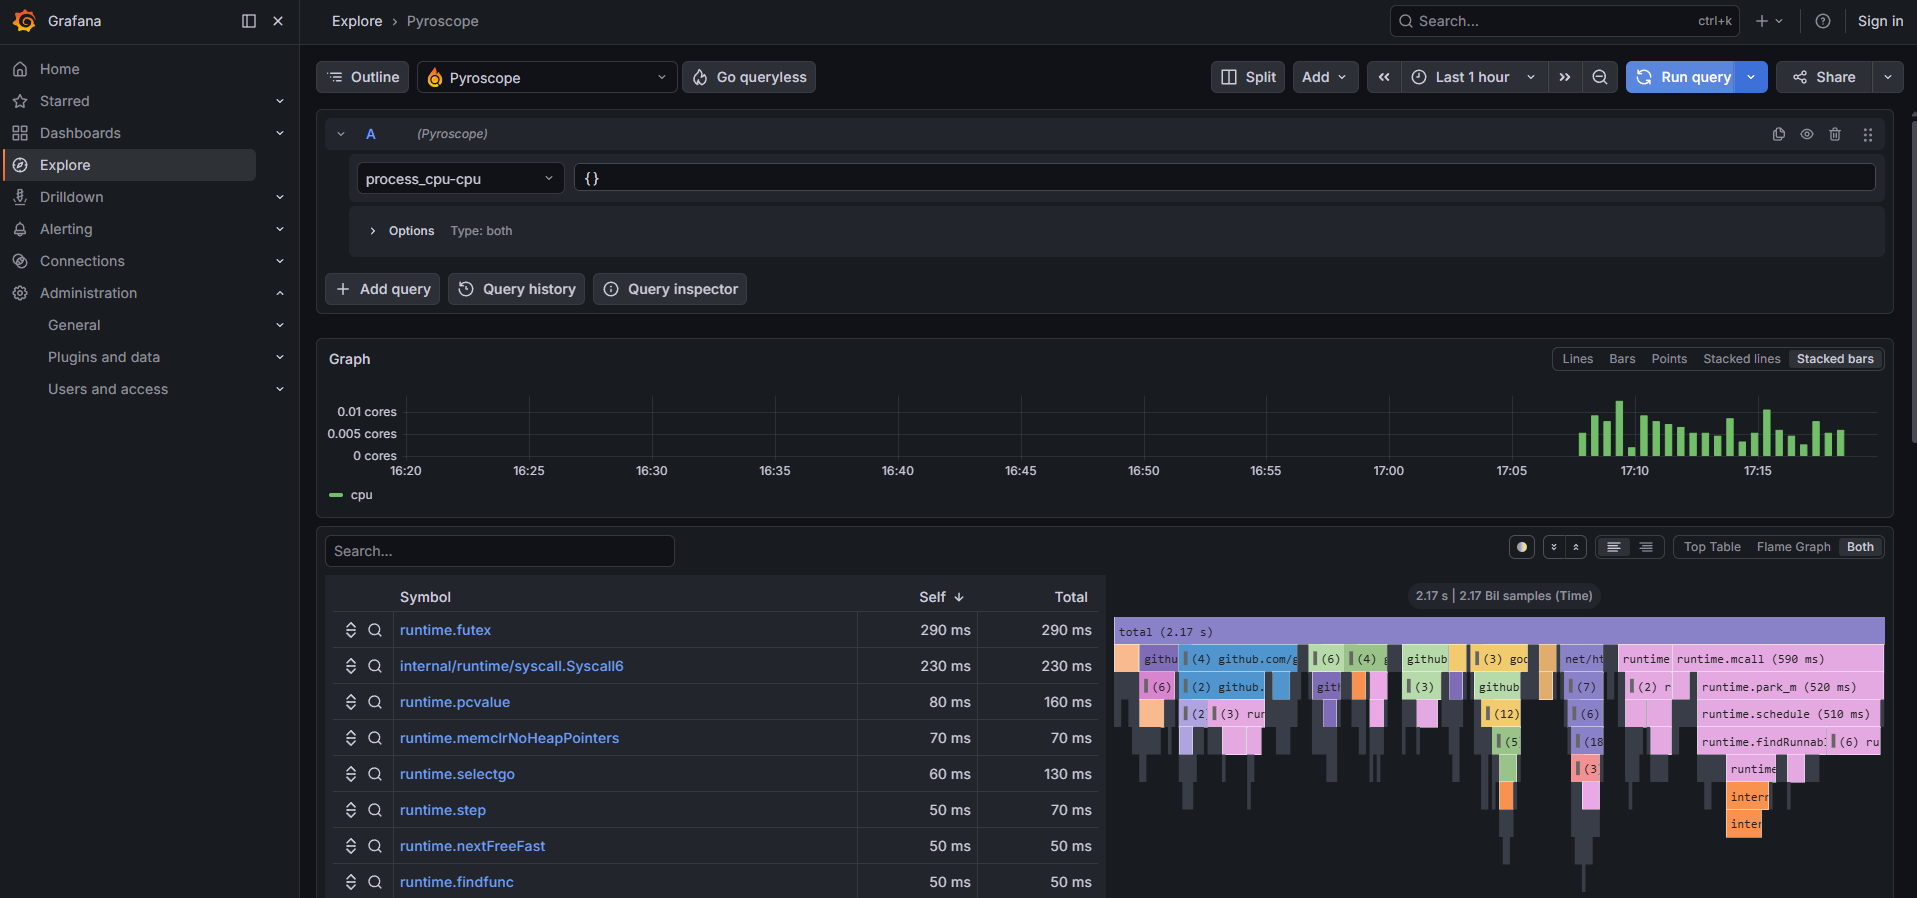
\includegraphics[width=0.9\textwidth]{figures/pyroscope.png}
    \caption{Pyroscope: flame graph de CPU del backend durante carga, permitiendo identificar cuellos de botella en el pipeline de inferencia.}
    \label{fig:pyroscope}
\end{figure}

% =============================================================================
% 5. DEMOSTRACION
% =============================================================================
\section{Demostraci\'on}
\label{sec:demo}

\subsection{C\'omo ejecutar el servicio}

El profesor puede levantar el servicio con un \'unico comando:

\begin{lstlisting}[language=bash, caption={Comando para ejecutar el servicio.}]
docker run --rm -p 8000:8000 ghcr.io/ahincho/chest-xpert-backend:latest
\end{lstlisting}

\noindent
Log esperado al arrancar:

\begin{lstlisting}[language={}, caption={Logs de arranque del servicio.}]
INFO: Loading ONNX model from models/chest-xpert-model.onnx
INFO: ONNX model loaded successfully
INFO: FilterService initialized with threshold=5.0
INFO: Uvicorn running on http://0.0.0.0:8000
\end{lstlisting}

\subsection{Ejemplo de solicitud}

Una vez arrancado, se puede enviar una radiograf\'ia al endpoint \texttt{/predict}:

\begin{lstlisting}[language=bash, caption={Request de ejemplo con curl.}]
curl -X POST http://localhost:8000/predict \
  -F "file=@radiografia_torax.png"
\end{lstlisting}

\subsection{Respuesta del modelo}

\begin{lstlisting}[language={}, caption={Response JSON real del servicio.}]
{
  "success": true,
  "predictions": [
    {"pathology": "Cardiomegaly",    "probability": 0.2543},
    {"pathology": "Edema",           "probability": 0.1606},
    {"pathology": "Consolidation",   "probability": 0.0134},
    {"pathology": "Atelectasis",     "probability": 0.0740},
    {"pathology": "Pleural Effusion","probability": 0.0610}
  ]
}
\end{lstlisting}

\subsection{Interpretaci\'on de resultados}

Cada valor en \texttt{predictions} es la probabilidad independiente ($\in [0, 1]$) de que la patolog\'ia est\'e presente en la radiograf\'ia. El modelo realiza clasificaci\'on multi-etiqueta, lo que significa que m\'ultiples patolog\'ias pueden estar presentes simult\'aneamente.

\begin{itemize}
    \item Valores $> 0.5$: alta sospecha de la patolog\'ia.
    \item Valores $\in [0.2, 0.5]$: sospecha moderada, requiere revisi\'on.
    \item Valores $< 0.2$: baja probabilidad.
\end{itemize}

El modelo est\'a dise\~nado como herramienta de \textbf{triaje}, no como diagn\'ostico definitivo. Debe utilizarse siempre bajo supervisi\'on de un profesional de salud.

\begin{figure}[H]
    \centering
    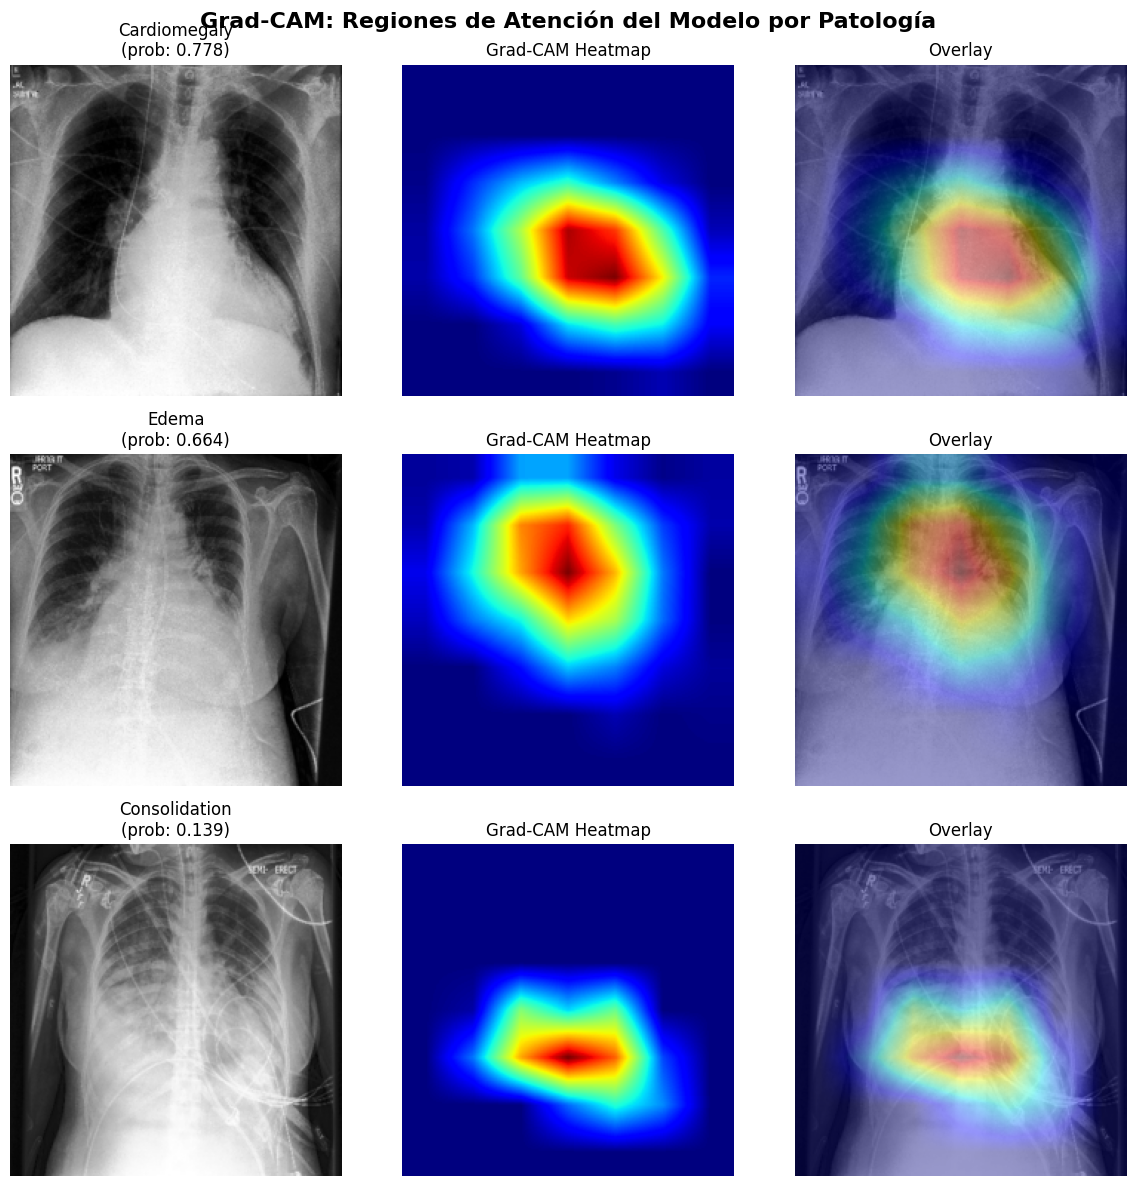
\includegraphics[width=0.85\textwidth]{figures/gradcam-cardiomegaly-edema-consolidation.png}
    \caption{Mapas Grad-CAM del modelo: Cardiomegaly (silueta card\'iaca), Edema (campos pulmonares) y Consolidation (opacidad focal). Atenci\'on anat\'omicamente correcta.}
    \label{fig:gradcam}
\end{figure}

\subsection{Respuestas de error}

El servicio maneja gracefully los errores:

\begin{itemize}
    \item \textbf{Imagen a color} (no radiograf\'ia): filtro RGB-Diff rechaza con mensaje descriptivo.
    \item \textbf{Archivo corrupto}: error 400 con mensaje ``Cannot decode image''.
    \item \textbf{Archivo demasiado grande} ($>$10MB): error 413.
    \item \textbf{Campo faltante}: error 422 con validaci\'on Pydantic.
\end{itemize}

% =============================================================================
% 6. CONCLUSIONES
% =============================================================================
\section{Conclusiones}
\label{sec:conclusions}

\subsection{Resumen de logros}

Se logr\'o desplegar exitosamente el modelo Chest Xpert AI como un servicio containerizado de producci\'on que cumple todos los criterios de la r\'ubrica:

\begin{enumerate}
    \item \textbf{Imagen Docker funcional}: arranca con un solo \texttt{docker run}, sin dependencias externas ni vol\'umenes.
    \item \textbf{Modelo funcional}: responde con predicciones correctas y pertinentes para las 5 patolog\'ias tor\'acicas.
    \item \textbf{Documentaci\'on clara}: README con instrucciones de construcci\'on, ejecuci\'on y ejemplo completo.
    \item \textbf{Pipeline CI/CD}: linting, testing, build y publicaci\'on autom\'atica en GHCR.
    \item \textbf{Versionado sem\'antico}: releases autom\'aticos basados en Conventional Commits.
    \item \textbf{Observabilidad}: stack LGTM completo con traces, logs, m\'etricas y profiling continuo.
\end{enumerate}

\subsection{Decisiones t\'ecnicas clave}

\begin{itemize}
    \item \textbf{ONNX Runtime sobre PyTorch}: reducci\'on de dependencias de $\sim$2GB a $\sim$50MB, manteniendo la misma precisi\'on del modelo con inferencia 10x m\'as r\'apida.
    \item \textbf{uv sobre pip}: resoluci\'on de dependencias 10--100x m\'as r\'apida, lockfile determinista que garantiza reproducibilidad bit-a-bit.
    \item \textbf{Modelo embebido en la imagen}: sacrifica tama\~no de imagen por simplicidad operativa. El profesor no necesita configurar nada.
    \item \textbf{Multi-stage build}: minimiza la superficie de ataque y el tama\~no final de la imagen al excluir herramientas de compilaci\'on.
\end{itemize}

\subsection{Lecciones aprendidas}

\begin{enumerate}
    \item \textbf{El shebang importa}: en builds multi-stage, los scripts del virtualenv quedan con rutas del builder stage. Soluci\'on: usar \texttt{python -m modulo} en vez de ejecutar el script directamente.
    \item \textbf{GITHUB\_TOKEN es suficiente para GHCR}: no se necesitan tokens personales para publicar im\'agenes en el Container Registry del mismo repositorio.
    \item \textbf{Semantic-release + GITHUB\_TOKEN no dispara workflows}: por dise\~no de GitHub. Los tags deben re-pushearse desde local o usar un PAT para triggear el CD.
    \item \textbf{Pinear versiones de Actions}: usar \texttt{v8} puede fallar si no existe el major tag; \texttt{v8.2.0} es m\'as seguro.
\end{enumerate}

\subsection{Trabajo futuro}

\begin{itemize}
    \item \textbf{Dashboards preconfigurados}: exportar dashboards de Grafana como JSON provisioning para despliegue autom\'atico.
    \item \textbf{Alertas}: configurar alertas en Grafana cuando la latencia p95 supere un umbral o el error rate suba.
    \item \textbf{Frontend containerizado}: la aplicaci\'on Angular servida desde Nginx como segunda imagen Docker.
    \item \textbf{Kubernetes}: despliegue con Deployment + Service + Ingress para escalabilidad horizontal.
    \item \textbf{Monitoreo de data drift}: alertas autom\'aticas cuando la distribuci\'on de entradas cambia respecto al training set.
    \item \textbf{Endpoint de explicabilidad}: Grad-CAM bajo demanda para interpretar predicciones individuales.
\end{itemize}


% --- Bibliography ---
\bibliographystyle{plainnat}
\bibliography{references}

\end{document}
